\documentclass{sig-alternate}
  \pdfpagewidth=8.5truein
  \pdfpageheight=11truein


\usepackage{graphicx,url} 
\usepackage{tikz}
\usepackage{times}
%\usepackage[dvips]{graphicx}
\usepackage{alltt} 
\usepackage{amsmath}
       
%Necess�rio para redefini��o do \cite.
\usepackage{ifthen}     
\usepackage{rotating}
\usepackage{hyperref}
%Ambiente matem�tico.
\usepackage{threeparttable} 

\usepackage{stmaryrd}
\usepackage{mathabx}
  
\usepackage[latin1]{inputenc} 
\newcounter{regraA}  
\setcounter{regraA}{1}
\newcommand{\regA}{(\theregraA) \addtocounter{regraA}{1}}

\newcounter{regraB}  
 \setcounter{regraB}{1}
 \newcommand{\reg}{(\theregraB) \addtocounter{regraB}{1}}
      
\sloppy 

\begin{document}
%
% --- Author Metadata here ---
\conferenceinfo{SAC'13}{March 18-22, 2013, Coimbra, Portugal.}
\CopyrightYear{2013} % Allows default copyright year (2002) to be over-ridden - IF NEED BE.
\crdata{978-1-4503-1656-9/13/03}  % Allows default copyright data (X-XXXXX-XX-X/XX/XX) to be over-ridden.
% --- End of Author Metadata ---

\title{\scalebox{2.5}{$\pi$}-PEWS: A Web Service Composition Language
Supporting Policies}
 
% \subtitle{[Extended Abstract]
% \titlenote{A full version of this paper is available as
% \textit{Author's Guide to Preparing ACM SIG Proceedings Using
% \LaTeX$2_\epsilon$\ and BibTeX} at
% \texttt{www.acm.org/eaddress.htm}}}
%
% You need the command \numberofauthors to handle the 'placement
% and alignment' of the authors beneath the title.
%
% For aesthetic reasons, we recommend 'three authors at a time'
% i.e. three 'name/affiliation blocks' be placed beneath the title.
%
% NOTE: You are NOT restricted in how many 'rows' of
% "name/affiliations" may appear. We just ask that you restrict
% the number of 'columns' to three.
%
% Because of the available 'opening page real-estate'
% we ask you to refrain from putting more than six authors
% (two rows with three columns) beneath the article title.
% More than six makes the first-page appear very cluttered indeed.
%
% Use the \alignauthor commands to handle the names
% and affiliations for an 'aesthetic maximum' of six authors.
% Add names, affiliations, addresses for
% the seventh etc. author(s) as the argument for the
% \additionalauthors command.
% These 'additional authors' will be output/set for you
% without further effort on your part as the last section in
% the body of your article BEFORE References or any Appendices.

\numberofauthors{5} %  in this sample file, there are a *total*
% of EIGHT authors. SIX appear on the 'first-page' (for formatting
% reasons) and the remaining two appear in the \additionalauthors section.
%
\author{
% You can go ahead and credit any number of authors here,
% e.g. one 'row of three' or two rows (consisting of one row of three
% and a second row of one, two or three).
%
% The command \alignauthor (no curly braces needed) should
% precede each author name, affiliation/snail-mail address and
% e-mail address. Additionally, tag each line of
% affiliation/address with \affaddr, and tag the
% e-mail address with \email.
%
% 1st. author
\alignauthor
Pl\'acido A. Souza Neto\\
	   \affaddr{Federal Institute of Rio Grande do Norte (IFRN)},\\
       \affaddr{Federal University of Rio Grande do Norte (UFRN)}\\
       \affaddr{Natal-RN, Brazil}\\
       \email{placido.neto@ifrn.edu.br}
\alignauthor Genoveva Vargar-Solar\\
       \affaddr{French Council of Scientific Research}\\
       \affaddr{LIG-LAFMIA }\\
       \affaddr{Saint Martin d'H\`{e}res, France}\\
       \email{Genoveva.Vargas-Solar@imag.fr}
\alignauthor Martin A. Musicante\\
       \affaddr{Federal University of Rio Grande do Norte (UFRN)}\\
       \affaddr{Natal-RN, Brazil}\\
       \email{mam@dimap.ufrn.br}
\and
\alignauthor Jos\'e-Luis Zechinelli-Martini\\
       \affaddr{Fundaci\'on Universidad de las Am\'ericas Puebla (UDLAP)}\\
       \affaddr{San Andr\'es Cholula, M\'exico}\\
       \email{joseluis.zechinelli@udlap.mx}
\alignauthor Valeria de Castro\\
       \affaddr{Universidad Rey Juan Carlos}\\
       \affaddr{M\'{o}stoles, Spain}\\
       \email{Valeria.deCastro@urjc.es}
}
% There's nothing stopping you putting the seventh, eighth, etc.
% author on the opening page (as the 'third row') but we ask,
% for aesthetic reasons that you place these 'additional authors'
% in the \additional authors block, viz.
\date{21 September 2012}
% Just remember to make sure that the TOTAL number of authors
% is the number that will appear on the first page PLUS the
% number that will appear in the \additionalauthors section.


\maketitle
\begin{abstract}
This paper presents an extension of  the PEWS language, named $\pi$-PEWS, for
reliably composing web services using \textit{policies}\footnote{properties
that the composition must obey.}. The expression of policies adds non functional
properties to service compositions, such as atomicity, persistence or QoS. A $\pi$-PEWS program defines the  behaviour of a compound web
service as the combination of individual operations and conditions for
expressing non-functional and temporal constraints. $\pi$-PEWS includes
constructs for defining non-functional properties by means of conditions, to be checked at
runtime. Therefore, a new runtime system for the language has been specified,
taking into consideration the verification of policies and temporal conditions.
% To the extent of our knowledge, the declarative expression of contracts in
% service compositions is novel; no composition language until now provides such
% constructs for expressing non-functional properties.            
\end{abstract}

% A category with the (minimum) three required fields
%\category{H.4}{Information Systems Applications}{Miscellaneous}
%A category including the fourth, optional field follows...
%\category{D.2.8}{Software Engineering}{Metrics}[complexity measures,
%performance measures]

%\terms{Delphi theory} 

\keywords{$\pi$-PEWS, Policy, Web Service, Specification Language}

%*********************************************************************************************************
\section{Introduction}
\label{sec:intro}
%*********************************************************************************************************

Service oriented programming has emerged as a new paradigm for building applications out of existing elements, the services, that export application programming interfaces (API) that are accessible on a network, for instance the Internet. 
According to this new paradigm, building an application is equivalent to express scripts that coordinate method calls to services in order to program its application logic. 
The Web services stack associates a set of standard models and  languages for representing messages  (SOAP), for defining service interfaces (WSDL), and service conversations (WSCL). 
The service based application can then be wrapped as a compound service, i.e., a service consisting of other services. 

Service based applications need to ensure a minimum level of reliability when exceptions come up or when they should provide security guarantees in the messages exchanged among services. 
The WS* family of languages~\cite{W3C} provides means for adding security, fault tolerance (atomicity) to services. 
The existence of all these languages results in complex specifications which are difficult to understand and to maintain, particularly when the application (i)  is composed of hundreds or thousands of services; (ii) deals with several non-functional properties~\cite{Dustdar05}. In the first case, it is not easy to respect and deal with service methods dependencies; and in the second case, the programer must implement and embed protocols in the service composition document and then use a runtime that can execute such protocols. 
 
The main goal of our work is to provide a declarative language that can address the expression of service compositions and non-functional properties for personalizing a service coordination behavior at execution time. 
Inspired by aspect-oriented approaches, the language with deal separately with service composition expression and non-functional properties in order to provide flexible service coordinations and encourage reuse and ease of maintenance.

This paper presents an extension of  the PEWS language, named $\pi$-PEWS, for reliably composing web services using policies. 
The expression of policies adds non functional properties to service compositions, such as atomicity, persistence or QoS.  
A $\pi$-PEWS program defines the  behaviour of a compound web service as the combination of individual operations and conditions for expressing non-functional and temporal constraints. 
$\pi$-PEWS adds new constructs for defining non-functional properties by means of conditions, to be checked at runtime. 

The remainder of the paper is organized as follows: Section~\ref{sec:pews} gives an overview of the PEWS language for expressing service interfaces and service compositions.
Section~\ref{sec:pewsContract-model} introduces the policy model that we propose for adding  non-functional properties and temporal constraints to service coordinations for personalizing  their behavior at execution time. 
Section~\ref{section:pewsgrammar} introduces $\pi$-PEWS an extension of PEWS for expressing policies. 
Section~\ref{sec:example}   describes a proof of concept showing the use of $\pi$-PEWS on a concrete example. 
Finally, Section~\ref{sec:conclusion} concludes the paper and discusses future work.

%...........................................................................................................................................
\section{Related work} 
%...........................................................................................................................................
 
The specification and implementation of non-functional properties for systems is a difficult problem. 
In general, middleware infrastructures have defined frameworks and libraries for programming such aspects but few languages and solutions address properties in an homogeneous way. 
A good example of this situation is the WS* standard family.  
For adding a transactional behaviour to a services' coordination it is necessary
to implement WS-Coordination, WS-Transaction, WS-BussinessActivity and
WS-AtomicTransaction. The WS-family addresses communication failures by
the WS-ReliableMessaging protocol \cite{ws-ra} which defines a protocol for
delivering messages in the presence of software component, system, or network failures. 

In \cite{schuldt-etal-TODS}, the authors use the WISE approach
\cite{alonso99wise,lazcano00wise} for making the state of each active process
persistent in an automatic way through a database, for recovering after system
failures. \cite{NepalFGJKS05} makes persistent any mission critical data to run
the business activities in a persistent storage. The data is accessed by the
code representing activities, and manipulated for further processing.
\cite{samy} uses the Bonita coordination engine \cite{Bonita} for providing
persistency to its coordinations. Each coordination is related to a project
which includes all the required information for recovering a given execution
point after a system failure. The selection of the adequate protocols for adding
a specific non functional properties to a service coordination (e.g., security,
transactional behaviour and adaptability) is responsibility of a programmer
\cite{Espinosa-OviedoVZC09}.
 

Behavior Specification Languages, such as Eiffel~\cite{Meyer98a}, JML~\cite{burdy:05} and IContract~\cite{LacknerKP02}, \textit{Graph Transformation} \cite{HL05TACoS, LeS92} and \textit{Transaction Specification Definition}
\cite{PiresBM02, Hernandez-BaruchPZ07, Haddad08} propose approaches for adding quality constraints to service composition. 
To the extent of our knowledge, the declarative expression of policies in
service compositions is novel; no composition language until now provides such
constructs for expressing non-functional properties.

% %...........................................................................................................................................
% \subsection{Contribution and organization of the paper} 
% %...........................................................................................................................................



%*********************************************************************************************************
\section{PEWS} \label{sec:pews}
%*********************************************************************************************************
 

PEWS\footnote{PEWS is an acronym of \textit{Path Expressions for Web
Services}.}~\cite{BaCAM05,BaAM06,MPC08} is a language for the
definition of web service interfaces. The language is devised to target the design of web services by specifying their \textit{behavior}, \textit{i.e,} the
relative order in which the operations of the service may be executed.

In a typical web service development setting, we have: \textit{(i)}\/ a WSDL document (defining the
operations of the service), \textit{(ii)}\/ a specification of the service semantics (possibly written in a natural
language) and \textit{(iii)}\/ a set of programs to implement each operation. 
Using those three elements, the service designer/programmer's task consists in producing some programs to implement the
specified semantics using the set of given programs.
The goal of PEWS is to be a programming language in which the service designer can combine the methods or subprograms that implement each operation of the service, in order to achieve the desired semantics.
A PEWS program acts as an upper layer for the set of programs implementing the data processing of the web service.
A PEWS program is also an extension to the web service interface defined as a WSDL document.
 
PEWS is based on the notion of \textit{predicate path expressions}~\cite{And79}.
This notion was introduced as a tool to express the synchronization of operations on data objects. 
Path expressions are programming language constructs used to restrict the 
allowable sequences of operations on an object. 
For instance, given the operations $a$, $b$ and $c$, the path expression 
$a*.(b || c)$ defines that the parallel execution of operations $b$ and $c$ 
should be preceded by zero or more executions of $a$. 

As noted in~\cite{And79}, the use of \textit{predicates} in path expressions allows a 
finer control of the access to the object being manipulated. 
For instance, the predicate path expression $a*.([P] b + [not P] c)$  
indicates that  either $b$ or $c$  would be executed  according to the 
truth-value of predicate $P$ (the execution of $b$ or of $c$ will be 
preceded by zero or more executions of $a$). 


The structure of a PEWS program is defined as~\cite{BaCAM05}:\\
\hrule
% \begin{displaymath}
% \begin{array}{rlr}
% \textit{Program} ::= & \ldbrack(\textrm{``} \mathbf{placido} \textrm{''} 
% \ldbrack(\textrm{``}\mathbf{placido} \textrm{''} & (1)\\
% 
% & \ldbrack(\textrm{``}\mathbf{placido} \ldbrack(\textrm{``}\mathbf{placido}
% \ldbrack(\textrm{``}\mathbf{placido}
% \textrm{''}
% \end{array}
% \end{displaymath}


\begin{tabbing}

\regA \textit{Program} ::=\=  \ $\ldbrack\ ($``$\mathbf{var}$''$\ \mathbf{id}\
$``$=$''$ \mathit{ArithExp} )^* $\\ \>$ \ ($``$\mathbf{service}$''$\
\mathbf{id}\ $``$=$''$ \mathit{Service})^* \ \mathit{Service}\ \rdbrack$\\[1.5mm]
\regA \textit{Service} ::=\=  \ $\ 	\ \ldbrack\  \mathbf{id} \ \rdbrack\
                                              \mid\ \ldbrack\ \mathit{Service}\
                                              $``$.$''$\ \mathit{Service} \
                                              \rdbrack\ $\\ \>$
                                              \mid\ \ldbrack\
                                              \mathit{Service} $``$+$''$\ \mathit{Service} \ \rdbrack\ $\\ \>$ \mid\ \ldbrack\  \mathit{Service} $``$\|$''$\ \mathit{Service} \ \rdbrack\
                                              \mid\ \ldbrack\  \mathit{Service}$``$*$''$\ \rdbrack\ $\\ \>$
                                              \mid \ \ldbrack\ $``$[$''$\
                                              \mathit{BooleanCondition}\
                                              $``$]$''$ \ \mathit{Service} \ \rdbrack\ $\\ \>$
                                              \mid\ \ldbrack\ $``$\{$''$\  \mathit{Service}\ $``$\}$''$\ \rdbrack\ $ \\[-3mm]
\end{tabbing}


\hrule

\vspace*{2mm}


\noindent According to the grammar above, a PEWS program $P$ is composed by a sequence of:
\begin{itemize}
\item Macro definitions: A variable $X$ is defined to
contain an arithmetic expression (\textit{ArithExp}). 
The value of a variable will be computed each time it is needed during the run of the program. 

\item Service definitions: Y is the name of the service defined by ``$\mathbf{service}\ Y = S$\/''.
 
\item A path expression (Service expression): Represents the service being 
defined by the program. 
Note that \textbf{id} can denote a service \textit{operation} (as defined in a WSDL document) or a service expression. 
A boolean condition can 
contain PEWS counters and variable identifiers.
The operators for constructing path expressions are similar to those of regular
expressions. 
The grammar for services, above, defines that a path expression can be a
WSDL-defined operation or a compound service, denoted by an identifier, the sequential ($\ . \ $) or parallel ($\ \| \ $) composition of services, the sequential ($*$)
or parallel ($\{\dots\}$) repetition of services or the conditional execution of a service ($[C]S$).
\end{itemize} 

% The language defines \textit{predicates on counters}:
% For each operation $O$ in the program, the PEWS runtime system implements 
% three counters, corresponding respectively, to the number of times the
% operation has been called (\texttt{req($O$)}), started (\texttt{act($O$)}) and ended
% (\texttt{term($O$)}). 
% Each of these counters is composed by a pair: natural number (the counter
% itself) and a timestamp, corresponding to the last time in which the counter 
% was modified.
% The \texttt{val} component of each counter represents the counter's value while
% the \texttt{time} component indicates the moment the counter
% was last modified.


The PEWS system \cite{MPC08} is formed by a front-end and a back-end.
The front-end is a WSDL-aware, syntax-directed editor for PEWS programs,
which is implemented as a plugin extension for the the Eclipse Platform.
The front-end includes a type checker and a generator of a XML representation of the PEWS programs. 

A prototype (proof of concept) implementation of the language has been built~\cite{BaH08}. 
In this tool, the execution of a PEWS program is based on graph transformation:
A dependence graph is generated from the source program and this graph is 
interpreted according to some reduction rules to evaluate the
service composition.


%*********************************************************************************************************
\section{Policies and Time Constraints} \label{sec:pewsContract-model}
%*********************************************************************************************************

% OLD TEXT (MARTIN - PLACIDO)
% In this section we extend the PEWS language to support the notion \textit{contract} and \textit{time constraints}. 
% The extension does not modify the syntax of existing PEWS programs, but complements it by specifying (non-functional) restrictions in a separate block.
% This feature is intended to enhance reusability and allows the programmer to adequate a program to specific requirements of the application being developed.
% This means that the program developer can reuse the control part of the program and add application-specific requirements as contract or time constraints.

% NEW TEXT (GENOVEVA - ZECHINELLI)

Behavioural web service interface languages describe not only the input/output interface of a web service but also the expected behaviour of its components. This behaviour can be specified as a workflow, defining the \textit{order} in which the components of a service will be executed, so that the workflow specifies the functional behaviour of the compound web service. This is what PEWS programs do.

Additionally, we can specify non-functional behaviour for a service;
\textit{i.e}, to impose some additional restrictions which are separated from
the general workflow of the service. This can be done by using the notion of
\textit{policy} to be added to each particular instantiation of the service.
The result of this is to allow a given service (workflow) to have different
restrictions in different contexts.

We extend the PEWS language to support the notion \textit{policy} including
\textit{time constraints}. The extension does not modify the syntax of existing
PEWS programs, but complements it by specifying (non-functional) restrictions in
a separate block. This feature is intended to enhance reusability and allows the
programmer to adequate a program to specific requirements of the application
being developed. This means that the program developer can reuse the control
part of the program and add application-specific requirements as policies.


%...........................................................................................................................................
\subsection{Policies} \label{sec:contract-model}
%...........................................................................................................................................

% TEXTO INSERIDO NA SECAO ANTERIOR - (GENOVEVA - ZECHINELLI)

% Behavioural web service interface languages describe not only the input/output interface of a web service but also the allowable behaviour of its components.
% This behaviour can be specified as a workflow, defining the \textit{order} in which the components of a service will be executed, so that the workflow specifies the functional behaviour of the compound web service.
% This is what PEWS programs do.
%  
% Additionally, we can specify non-functional behaviour for a service; \textit{i.e}, to impose some additional restrictions which are separated from the general workflow of the service. 
% This can be done by using the notion of \textit{contract} to be added to each particular instantiation of the service.
% The result of this is to allow a given service (workflow) to have different restrictions in different contexts.

The model of policy proposed here follows the main ideas presented
in~\cite{Espinosa-OviedoVZC09, PortillaHE08}, where policies\footnote{In
\cite{PortillaHE08}, this concept is colled ``\textit{contract}''.} are added to
a given composition, as a separate concern. The properties defined by a policy
should be verified at runtime. Recovery actions, defined by the contract, are to
be performed in case of failure of the contract's conditions. Recovery actions
are defined by the policy itself. The proposals of~\cite{Espinosa-OviedoVZC09,
PortillaHE08} complement the previous work with PEWS, adding a new dimension to
the definition of web services. Similar services, sharing the same workflow, can
be specialized to individual applications, by defining different contracts for
each of them.


The policy model is defined to ensure runtime reliability  properties such as
exception handling, persistency, security, and atomicity. When these properties
are not verified, an exception is raised and recovery actions can be taken.
Policies can be used to associate a \textit{personalized behavior} to a workflow
describing the application logic of services based applications. The policy
model assumes that given a service coordination described by a workflow it is
possible to associate personalized properties to it in an orthogonal way. This
approach for defining non-functional properties helps to decouple the
application logic from its properties thereby encouraging the reuse of
coordinations and contracts. The same application logic can have two different
sets of contracts depending on its use. For example a service can require two
different security policies depending on the type of network from which it is
accessed.


% A policy is identified by a \textit{name} and it is applied to an
% \textit{execution unit}, which can be an application logic expressed as a
% \textit{workflow}, or an \textit{operation}.  It defines some
% \textit{properties} to be verified by the contract implementation. Each
% property, has a  \textit{scope} that defines the interval  in which the property
% can be verified, and a \textit{recovery strategy}, to define recovery actions
% when the property is not verified. Recovery actions include the substitution of
% the failed service for an equivalent one or roll back the coordination to the
% point before the failure.       


%...........................................................................................................................................
\subsection{Time Constraints}
\label{proposal:temporalModel}
 %...........................................................................................................................................

% OLD TEXT (MARTIN - PLACIDO) 
% The model of time relations proposed here follows the main ideas presented in
% \cite{Allen83}.
% This model is used to add new restrictions to the composition of web services over time. 
% The model will be used to impose additional restrictions to the order in which operations of a web service will be performed.

% NEW TEXT (GENOVEVA - ZECHINELLI)
The model of temporal relations proposed here follows the main ideas presented in
\cite{Allen83, BeVaC00}. The model is used to impose additional restrictions to
the order in which operations of a web service are performed at execution time.
For example, ``the confirmation of a bank authorization request must arrive at
most one minute after the service call''.


%The temporal relations presented here aims a better coordination for web services
%process. 
%This proposal presents an initial concern to coordinate services based on
%relation between services, such as \textit{before, start, overlap,
%etc}. 
 
A service composition time relation is represented by the following
model: Let   $\Omega$ be a set of web services ($\omega_1$, . . .,
$\omega_n$) to be composed and $\Theta$, a set of temporal relations $r_t$ that can be applied to $\Omega$. 
Temporal relations are defined by predicates $r_t:\ \Omega$ x $\Omega$, where
$r_t \in$~\{\textbf{\textit{none, before, meet, overlap, start, during, finish, equal}}\}. 
For example, the following expression defines that the operation $\omega_1$ needs to be finished before the operation $\omega_3$ is alllowed to start: 
\textbf{\textit{before($\omega_1, \omega_3$)}}.  
The expression \textbf{\textit{meet(before($\omega_1, \omega_3$)$, \omega_2$)}} states that the execution of operation $\omega_2$ will begin as soon as $\omega_3$ finishes and that $\omega_3$ can begin any time after $\omega_2$ stops.



Additionally, we can define general, sequential and parallel restrictions (named, respectively, \textbf{\textit{seq}} and \textbf{\textit{par}}), as well as the inverse relations for each of the relations defined above. 
The inverse relations will be named, respectively, \textbf{\textit{Ibefore}}, \textbf{\textit{Imeet}}, \textbf{\textit{Ioverlap}}, \textbf{\textit{Istart}}, \textbf{\textit{Iduring}} and their semantics is the same as the original relations, but with their arguments swapped.

%*********************************************************************************************************
\section{$\pi$-PEWS} 
\label{section:pewsgrammar}
%*********************************************************************************************************

Let us now define the policies in PEWS, using the concepts described in the previous subsections.
$\pi$-PEWS extends PEWS programs with the notion of policy.
$\pi$-PEWS policies can contain conditions to be checked at runtime, as well as temporal restrictions.
The model of policies presented here is inspired on successful contract models,
like the ones used by JML~\cite{burdy:05} and JCML~\cite{jcml09,daCosta2010}.

$\pi$-PEWS policies will specify assertions that will be checked during the
execution of a composition. These assertions describe pre- and post-conditions for a given operation or compound service.
In the case these conditions are not verified, the policy can define
\textit{correcting actions} (described as a PEWS path expression). Temporal
restrictions can also be defined within a policy.
 
%Works try to adapt some tools and
%approaches aiming add quality constraints, like \textit{Behavioral Specification
%Language}, such as: Eiffel~\cite{Meyer98a}, JML~\cite{burdy:05}, JCML~\cite{jcml09} and
%IContract~\cite{LacknerKP02}, \textit{Graph Transformation}
%\cite{HL05TACoS, LeS92} and \textit{Transaction Specification Definition}
%\cite{PiresBM02, Hernandez-BaruchPZ07, Haddad08} for service composition.
%However, none of than proposes a hole application of service composition and
%behavioral specification definition for web services. 

A $\pi$-PEWS program is similar to a PEWS program, but with the possibility of adding policy definitions at the end of the program.
Path expressions, defining the service workflow, are described by the \textit{Service} nonterminal of the grammar below. 
Since policies and workflow are separate concerns, the syntax of path expressions remain unchanged, from the original version of the language.\\
\hrule
\begin{tabbing}
\reg \textit{Program} ::=\=  \ $\ldbrack\ ($``$\mathbf{var}$''$\ \mathbf{id}\
$``$=$''$ \mathit{ArithExp} )^* $\\ \>$ \ ($``$\mathbf{service}$''$\
\mathbf{id}\ $``$=$''$ \mathit{Service})^* \mathit{Service}\ \mathit{Policy}^ *\
\rdbrack$\\[1.5mm] \reg \textit{Service} ::=\=  \ $\ 	\ \ldbrack\  \mathbf{id} \ \rdbrack\ \mid\ \ldbrack\ \mathit{Service}\
                                              $``$.$''$\ \mathit{Service} \ \rdbrack\ $\\ \>$
                                              \mid\ \ldbrack\ \mathit{Service} $``$+$''$\ \mathit{Service} \ \rdbrack\ $\\ \>$
                                              \mid\ \ldbrack\  \mathit{Service} $``$\|$''$\ \mathit{Service} \ \rdbrack\ 
                                              \mid\ \ldbrack\  \mathit{Service}$``$*$''$\ \rdbrack\ $\\ \>$
                                              \mid \ \ldbrack\ $``$[$''$\
                                              \mathit{BooleanCondition}\ $``$]$''$ \ \mathit{Service} \ \rdbrack\ $\\ \>$
                                              \mid\ \ldbrack\ $``$\{$''$\  \mathit{Service}\ $``$\}$''$\ \rdbrack\ $ \\[-3mm]
\end{tabbing}
\hrule
\vspace*{2mm}

The definition of policies is given below. 
It includes a name for the policy, as well four component sections:
\begin{itemize}
\item Target service of the policy: This section specifies the service to which the policy applies. This can be an operation or a compound service (which also defines a scope for the policy).
\item Pre-conditions and their actions. This section defines the assertions that will be verified before the target service is executed. 
\item Post-conditions and their actions. This section defines the assertions that will be verified at the end of the target service execution. 
\item Time constraints for the services on the policy scope.
\end{itemize} 

\bigskip

\hrule


\begin{tabbing}
\reg \textit{Policy} ::= \= $\ldbrack$ ``\textbf{def} '' ``\textbf{policy}'' 
\textit{Id}  ``\textbf{\{}'' \\
  \>  \textit{IsAppliedTo}  
  \textit{Requires*}
  \textit{Ensures*} \\
\>   \textit{(TimeConstraint)?} ``\textbf{\}}'' $\rdbrack$\\[-3mm]
\end{tabbing}


\hrule
\vspace*{2mm}

The directive ``\textbf{isAppliedTo:}'' defines the target service and scope of the policy. 
This service is given by the identifier appearing next to the keyword.
The target service can be a simple operation or a compound service. 
In the former case, the policy cannot contain any time restriction.
In the case of a policy defined for a compound service, the operations and services that form the policy can participate of the time constraint expressions defined by the policy.\nopagebreak\\
\hrule
\begin{tabbing}
 \reg \textit{IsAppliedTo} ::= \= $\ldbrack$ ``\textbf{isAppliedTo}''
  ``\textbf{:}''  \textit{ident} ``\textbf{;}'' $\rdbrack$ \\[-3mm]
  \end{tabbing}
\nopagebreak\hrule\nopagebreak
\vspace*{2mm}

The ``\textbf{requires}'' and ``\textbf{ensures}'' parts of a policy define the
pre-conditions (resp. post-conditions) to be checked for each of them. In the
case of pre-conditions, they will be verified before the service is executed. Post-conditions will be checked after the execution of the service.
In both cases, when the assertion fails, the associated action will be executed.
Actions are defined as services, and written as PEWS path expressions.\\

\hrule
\begin{tabbing}
\reg \textit{Requires} ::= \= $\ldbrack$ ``\textbf{requires}''
  \textit{BooleanCondition} \textit{(} \\  \>   ``\textbf{(}''
  \textit{onFailureDo} ``\textbf{)}'' \textit{)?} ``\textbf{;}'' $\rdbrack$
  \\[1.5mm]
  
   \reg \textit{Ensures} ::= \= $\ldbrack$ \textbf{`ensures'}
  \textit{BooleanCondition} \textit{(} \\  \>  ``\textbf{(}''
  \textit{onFailureDo} ``\textbf{)}'' \textit{)?} ``\textbf{;}'' $\rdbrack$
  \\[1.5mm]
  
   \reg \textit{onFailureDo} ::= \= $\ldbrack$ \textbf{`onFailureDo'}
  \textit{Service} $\rdbrack$ \\[-3mm]
\end{tabbing}
\hrule
\vspace*{2mm}

Time Constraints are defined as relational expressions build from the operators presented in section~\ref{proposal:temporalModel}. 
These constraints will be imposed to the execution of the composition.\\


\hrule
\begin{tabbing}
  
  \reg \textit{timeConstraint} ::= \= $\ldbrack$
  \textbf{`timeConstraint'} \textbf{`:'} \textit{timeRelation} \textbf{`('} \\ \>
  (\textit{opName} $|$ \textit{timeConstraint}) \textbf{`,'} \\ \> (\textit{opName} $|$ \textit{timeConstraint}) \textbf{`)'} \\ 
   \> $\rdbrack$ 
  \\[1.5mm] 
  
   \reg \textit{timeRelation} ::= \= $\ldbrack$  ``\textbf{before}'' $\rdbrack$ 
   $|$ $\ldbrack$  ``\textbf{meet}'' $\rdbrack$ $|$
   $\ldbrack$  ``\textbf{start}'' $\rdbrack$ \\  \> $|$
   $\ldbrack$  ``\textbf{overlap}'' $\rdbrack$ $|$ 
   $\ldbrack$  ``\textbf{during} $\rdbrack$ $|$ $\ldbrack$  ``\textbf{finish}''
   $\rdbrack$ \\  \>  $|$ $\ldbrack$  ``\textbf{equals}'' $\rdbrack$ $|$ 
   $\ldbrack$ ``\textbf{Ibefore}'' $\rdbrack$ $|$  $\ldbrack$ ``\textbf{Imeet}'' $\rdbrack$ 
   \\  \>  $|$ $\ldbrack$ 
   ``\textbf{Istart}'' $\rdbrack$ $|$ $\ldbrack$ 
   ``\textbf{Ioverlap}'' $\rdbrack$  $|$ $\ldbrack$ 
   ``\textbf{Iduring}'' $\rdbrack$ \\[-3mm]
\end{tabbing}
\hrule
\vspace*{2mm}
\bigskip 


\subsection{$\pi$-PEWS Meta-model}

$\pi$-PEWS is intended to be the implementation language of a
model-driven development method called $\pi$SOD-M~\cite{submited}. This
section presents the meta-model that corresponds to the implementation (platform-specific model)
of the $\pi$SOD-M method.

The $\pi$-PEWS meta-model is based on the service composition
approach provided by the language $\pi$-PEWS, a programming language that lets
the service designer combine the methods or subprograms that implement
operation and policies of a service, in order to achieve the desired application
logic. Figure \ref{fig:metamodel} presents the $\pi$-PEWS meta-model consisting
of  classes representing:   


\begin{figure}
\centering
\fbox{
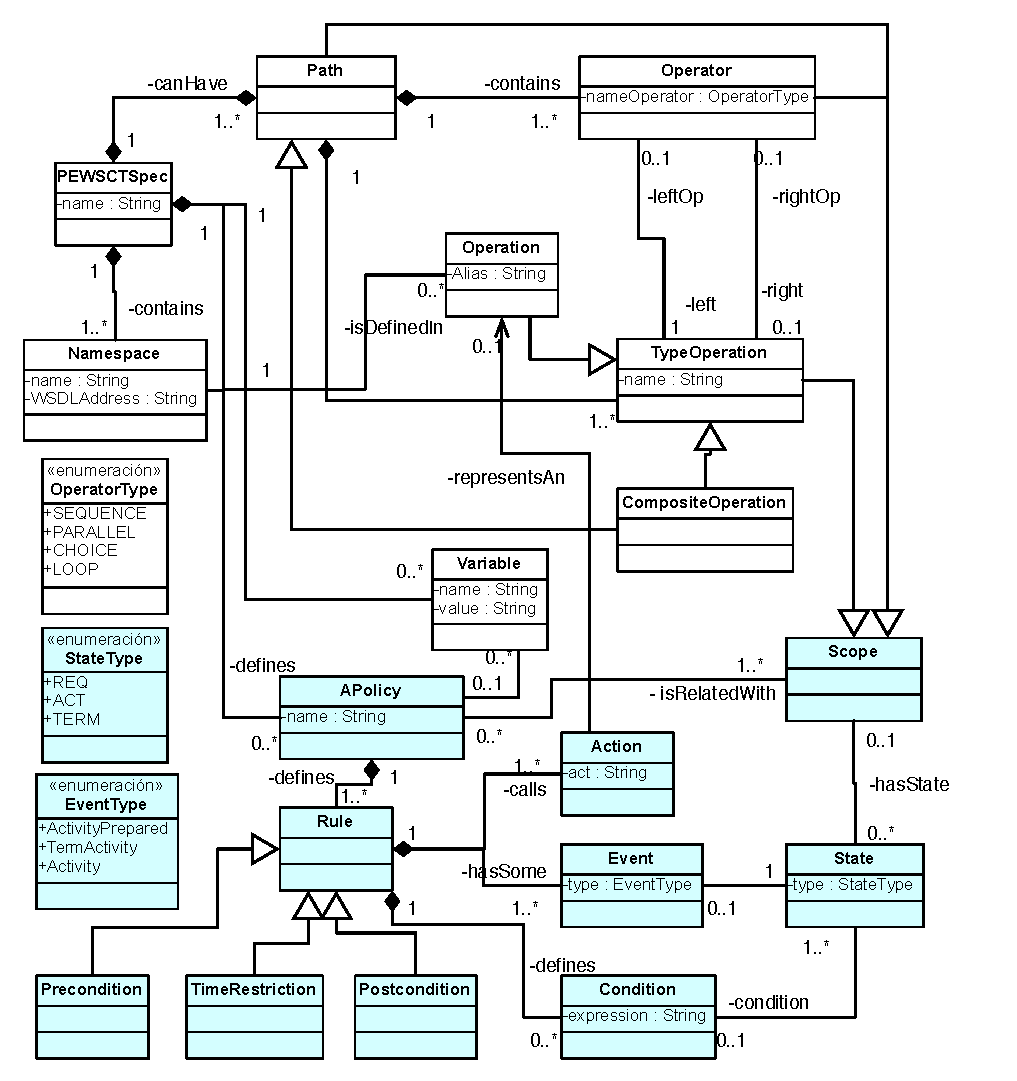
\includegraphics[width=.45\textwidth]{figs/PiPEWSMetamodel.pdf}
}
\caption{$\pi$-PEWS Meta-model.}
\label{fig:metamodel}
\end{figure} 

\begin{itemize}
\item A service composition: {\sc Namespace} representing the interface exported
by a service; {\sc Operation} that represents a call to a service method, {\sc
CompositeOperation}; and  {\sc Operator} for representing a service composition
and {\sc Path} representing a service composition. A {\sc Path} can be an {\sc
Operation} or a {\sc Compound Operation} denoted by an identifier. A {\sc
Compound Operation} is defined using an  {\sc Operator}  that can be represent 
sequential ($\ . \ $) and parallel ($\ \| \ $) composition of services, choice
($\ + \ $) among services, the sequential ($*$) and parallel ($\{\dots\}$)
repetition of an operation or the conditional execution of an operation ($[C]S$).

\item {\em A-Policies} that can be associated to a service composition:  {\sc
A-Policy}, {\sc Rule}, {\sc Event}, {\sc Condition}, {\sc Action}, {\sc State},
and {\sc Scope}.
\end{itemize}
%     

As shown in the diagram (figure \ref{fig:metamodel}) an {\sc A-Policy} is
applied to a {\sc Scope} that can be either an {\sc Operation} (e.g., an authentication protocol associated to a
method exported by a service), an {\sc Operator} (e.g., a temporal constraint
associated to a sequence of operators), and
a {\sc Path}. An {\sc A-Policy} groups a set of ECA rules \cite{PortillaHE08}:
each rule having a classic semantics, i.e, {\em when an event of type E occurs if  condition C is
verified then execute the action A}.  Thus, an {\em A-policy} represents a set
of reactions to be possibly executed if one or several triggering events of its
rules are notified.
\begin{itemize}
\item The class {\sc Scope} represents any element of a service composition
(i.e., operation, operator, path).
\item The class {\sc A-Policy} represents a recovery strategy implemented by ECA
rules of the form {\sc Event} - {\sc Condition} - {\sc Action}. An {\em
A-policy} has variables that represent the view of the execution state of its associated
scope, that is required for executing the rules. The value of a variable is
represented using the type {\sc Variable}. The class {\sc A-Policy} is
specialized for defining specific constraints, for instance authentication {\em
A-policies}.
\end{itemize}


% The grammar in this section defines the extension for the PEWS language, to
% include policies and time constraints. 
In the next section we use $\pi$-PEWS to show how a composition with additional
requirements can be modeled by our language.

%*********************************************************************************************************
\section{$\pi$-PEWS in Action: An example of web services composition} \label{sec:example}
%*********************************************************************************************************
 
\begin{figure}
\centering

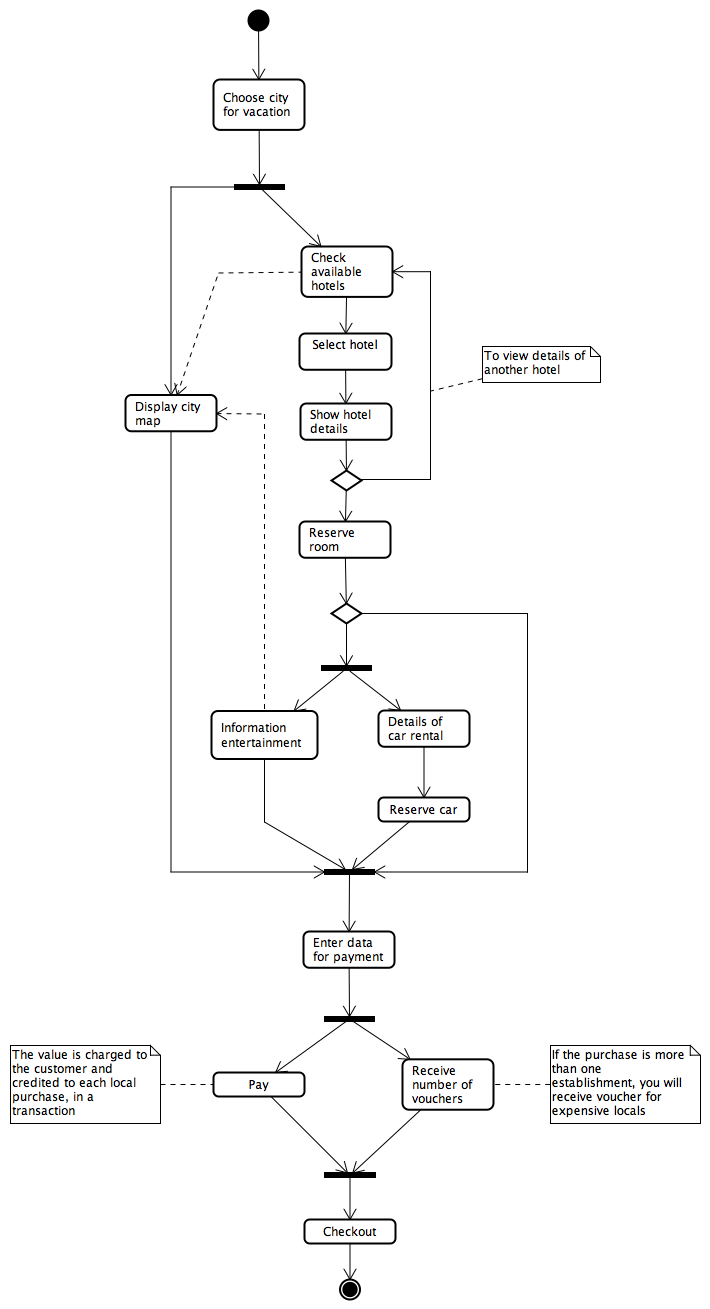
\includegraphics[width=.5\textwidth]{figs/proofConcept.png}

\caption{Business Process Definition Example.}
\label{fig:example}
\end{figure}

This case study presents a classic example in a web service composition. It
is an example for booking hotels, car and entertainment activities for people
who want to take vacations. Web sites usually offer web services for booking hotels, cars and entertainment activities. For this example users can choose a desired city and look for
hotels availability. Then, if the user is interested in a
hotel, the accommodation service can be called for booking it. After
choosing  accommodation, the user can also search for entertainment
programs, such as museums and festivals, always with the service map
location to show the city map. In parallel, the user also can search for car
rental agencies and finally pay for that services and receive a
booking receipt. Figure~\ref{fig:example} shows an activity diagram for the business process example.
There is a total of 13 operations in the process.
The implementation of these operations will communicate using SOAP messages that encapsulate the input
and output parameters.

\begin{figure}[ht]
\centering
\tiny
\begin{verbatim}
1 ns namespaceA = "http:\\www.dimap.ufrn.br/MapsService.wsdl"
2 ns namespaceB = "http:\\www.dimap.ufrn.br/HotelInformationService.wsdl"
3 ns namespaceC = "http:\\www.dimap.ufrn.br/CarRentalService.wsdl"
4 ns namespaceD = "http:\\www.dimap.ufrn.br/Entertainment;Service.wsdl"
5 ns namespaceE = "http:\\www.dimap.ufrn.br/BankService.wsdl"

6  alias chooseCity(in) = portType/chooseCity in namespaceA
7  alias showMap(in,out) = portType/showMap in namespaceA
8  alias searchHotel(in,out) = portType/searchHotel in namespaceB
9  alias hotelInformation(in,out) = portType/hotelInformation in namespaceB
10 alias selectHotel(in,out) = portType/selectHotel in namespaceB
11 alias viewDetails(out) = portType/viewDetails in namespaceB
12 alias reservationRoom(in,out) = portType/reservationRoom in namespaceB
13 alias entertainmentsView(in,out) = portType/entertainmentsView in namespaceD
14 alias searchCarRental(in,out) = portType/searchCarRental in namespaceC
15 alias reservationCar(out) = portType/reservationCar in namespaceC
16 alias setDataPayment(in) = portType/setDataPayment in namespaceE
17 alias payment(in,out) = portType/payment in namespaceE
18 alias getVoucherNumber(out) = portType/getVoucherNumber in namespaceE
19 alias checkout(out) = portType/checkout in namespaceE

20 service hotelLookup = (searchHotel . selectHotel . viewDetails)*
21 service hotelReservation = hotelLookup . reservationRoom
22 service payAndGetVoucher = payment  ||  getVoucherNumber

23   chooseCity . (showMap ||
24                  (hotelReservation  |
25                   hotelReservation  .
26                    (entertainmentsView  ||
27                     (searchCarRental  .  reservationCar )
28                    )
29                  )
30                ) .
31   setDataPayment  .  payAndGetVoucher   .
32   checkout
\end{verbatim}

\caption{$\pi$-PEWS Specification (1).}
\label{fig:examplepewscontract}
\end{figure}


The $\pi$-PEWS program that implements this service is given in Figures~\ref{fig:examplepewscontract} and~\ref{fig:examplepewscontract2}.
In these figures, lines 1 to 5 define the location of the web services to be used by the composition.
Lines 6 to 19 associate identifiers in the program for each operation exposed by
the WSDL documents and being used to form the compound service. These lines also states the input-output behaviour of each individual operation.
Lines 20 to 22 define sub-services to be used in the composition. The identifiers bound by these definitions can be used to build complex services, as well as to define policies for them.

Lines 23 to 32 of Figure~\ref{fig:examplepewscontract} define the workflow for
the reservation service. This workflow corresponds to the diagram in Figure~\ref{fig:example}.


%Figure \ref{fig:example} shows the activity diagram for
%the business process example. There are 13 operations in the hole process. Following the sequence of
%operations for the \textit{travel operations} is listed.
%
%\begin{itemize}
%  \item Travel Workflow Operations:
%\begin{itemize}
%  \item \textbf{\textit{chooseCity}}: Choose city for vacation;
%  \item \textbf{\textit{showMap}}: Display city map;
%  \item \textbf{\textit{searchHotel}}: Check available hotels;
%  \item \textbf{\textit{selectHotel}}: Select hotel;
%  \item \textbf{\textit{viewDetails}}: Show hotel details;
%  \item \textbf{\textit{reservationRoom}}: Reserve room;
%  \item \textbf{\textit{entertainmentsView}}: Information entertainment;
%  \item \textbf{\textit{searchCarRental}}: Details of car rental;
%  \item \textbf{\textit{reservationCar}}: Reserve car;
%  \item \textbf{\textit{setDataPayment}}: Enter data for payment;
%  \item \textbf{\textit{payment}}: Pay;
%  \item \textbf{\textit{getVoucherNumber}}: Receive number of vouchers;
%  \item \textbf{\textit{checkout}}: Checkout.
%\end{itemize}
%\end{itemize}

The policy part of the $\pi$-PEWS program is defined in Figure~\ref{fig:examplepewscontract2}.
This part of the program defines two policies.
The first policy will be applied to the service identified by \texttt{hotelLookup}.
Its pre-condition states that the input string to be passed to the \texttt{searchHotel} operation as its input parameter is not empty.
The failure of this condition triggers the \texttt{hotelInformation} operation, which is an alternative hotel search service.
The post-condition of this policy ensures that one hotel was found.
This policy specify an additional restriction to the workflow, imposing that the \texttt{viewDetails} operation is executed right after \texttt{selectHotel} finishes.


The second policy (\texttt{policy02}, specified by lines 40 to 48 in
Figure~\ref{fig:examplepewscontract2}) is applied to the component service named \texttt{payAndGetVoucher} (defined in Figure~\ref{fig:examplepewscontract}). Its precondition states that a positive amount of money is to be used as payment for the reservation and that this value is the value agreed for the service.
The precondition also sets a restriction on the number of times this operation can be retryed: More than 3 requests for the \texttt{payment} operation will result on the abortion of the whole process.
The post-condition of this policy states that the payment operation is successful and that a non-null voucher number is produced to be communicated to the user.
The time restriction associated to the policy states that the \texttt{getVoucherNumber} operation will be initiated during the \texttt{payment} verification.

\begin{figure}
\centering
\tiny
\begin{verbatim}
33 def policy policy01{
34   isAppliedTo: hotelLookup;
35   requires: searchHotel@in != null
36      (onFailureDo hotelInformation); // alternative hotel search engine
37   ensures:  searchHotel@out.Length > 0;
38   timeConstraint : meet(selectHotel, viewDetails);
39 }

40 def policy policy02{
41   isAppliedTo: payAndGetVoucher;
42   requires: payment@in == setDataPayment@in && payment@in > 0
43             && req(payment).val <= 3
44      (onFailureDo abortOperation);
45   ensures:  payment@out == true && getVoucherNumber@out != null
46        (onFailureDo throw PaymentException);
47   timeConstraint : overlap(payment, getVoucherNumber);
48 }
\end{verbatim}
\caption{$\pi$-PEWS Specification (2).}
\label{fig:examplepewscontract2}
\end{figure}

An prototype implementation of the environment to code $\pi$-PEWS specification 
have been produced in the form of a plugin for the Eclipse platform.

%*********************************************************************************************************
\section{Conclusion and future work}\label{sec:conclusion} 
%*********************************************************************************************************

%% OLD TEXT (MARTIN - PLACIDO)
% The coordination of web services is a complex task~\cite{MorseBPMTM04, KoutsoukosKANS06, pullen09, ChengGCM09}.
% Along the last years, a number of languages and tools to support of the development of web services have been devised.
% Traditional software engineering methods should be adapted to this kind of systems.
% Existing approaches do not provide a quick and robust support for the efficient development
% of complex web service applications (where functional and nonfunctional requirements have to be considered).
% Thus, the design, implementation and test phases become more complex and expensive.
% The extension of PEWS presented in this paper was aimed to provide a more
% integrated systems development that use the service composition, in which it is
% possible besides specifying process flow for the services implementation,
% quality requirements and behavior can also be described in the PEWS language.
% 
% We postulate that the new primitives are adequate to express conditions to  related to properties related to the quality of the service being defined

%% NEW TEXT (GENOVEVA - ZECHINELLI)
% Coordinating web services is a complex task~\cite{MorseBPMTM04, KoutsoukosKANS06, pullen09, ChengGCM09}.
% During the last years, a number of languages and tools to support of the development of web services have been proposed.
% Existing approaches do not provide a declarative and robust support for the efficient development
% of complex web service applications where functional and nonfunctional requirements have to be considered.
% The extension of $\pi$-PEWS presented in this paper provides an 
% integrated approach for programming service compositions by 
%  specifying the control flow of service compositions and their associated
% quality requirements and behavior.
% 
% \ldots
%  
% \ldots 
%  
% 
% $\pi$-PEWS aims to be the beginning for an integrated solution proposal for
% web services composition development. The language extension also aims to search
% for a more robust solution for distributed developing applications, serving as a
% subsidy for a more systematic development of
% software, and thus direct ourselves towards addressing one of the issues
% described in the Grand Challenges in Computer Science.
 
%% NEW TEXT (GENOVEVA - ZECHINELLI)
Coordinating web services is a complex task~\cite{MorseBPMTM04, KoutsoukosKANS06, pullen09, ChengGCM09}.
During the last years, a number of languages and tools to support of the development of web services have been proposed. 
Existing approaches do not provide a declarative and robust support for the efficient development of complex web service applications where functional and nonfunctional requirements have to be considered.
The extension of PEWS presented in this paper provides an integrated approach for programming service compositions by specifying the control flow of service compositions and their associated temporal requirements and behaviour. 
Both temporal and behaviour requirements can be used to define the quality of service and the reliability of the composition. 
$\pi$-PEWS proposes an integrated solution for web services composition development. 
The language extension can provide a  robust solution for distributed service based applications which is important to ensure the correctness of services compositions particularly when they have to scale to many services. 
Following the service-oriented programming philosophy of ease of construction of
distributed applications, $\pi$-PEWS provides a way of programming applications
declaratively ($\pi$-PEWS plugin for Eclipse), and encourages the separation of
the application logic and non-functional aspects specification.

We are currently working on a verification approach that can ensure $\pi$-PEWS programs correctness. 
We are also extending the $\pi$-PEWS runtime in order to compile policies and
generate code for reliable services coordinations. 

% Finally, we will develop proofs of concepts for services mashups applied to
% e-government applications in the context of the project e-CLOUDSS (e-cloudss.imag.fr).
%   
  
%$\pi$-PEWS aims to be the beginning for an integrated solution proposal for
%web services composition development. The language extension also aims to search
%for a more robust solution for distributed developing applications, serving as a
%subsidy for a more systematic development of
%software, and thus direct ourselves towards addressing one of the issues
%described in the Grand Challenges in Computer Science.
% 
% %*********************************************************************************************************
% \section{Aknowledgements} 
% %*********************************************************************************************************
% This work is partially financed by the Microsoft LACCIR e-CLOUDSS project
% developed with UFRN, Brazil, U. de la Republica, Uruguay, and UDLAP, Mexico (http://e-cloudss.imag.fr).
% 
%    
\bibliographystyle{abbrv}
\bibliography{biblio}


\end{document}
